\section{Performance Analysis}
The simulation was implemented in a Python environment based on the open-source \texttt{physio-key-gen} repository \cite{physiokeygen}. The implementation uses the \texttt{wfdb} library to process real medical ECG data from the MIT-BIH Arrhythmia Database (Record 103) \cite{mitbih}, distributed through PhysioNet \cite{goldberger2000physionet}. Keys are derived with SHA-1 and verified with HMAC, and an execution time tracker measures the computational cost of the algorithm. Table~\ref{tab:params} lists the parameters used.

\begin{table}[htbp]
  \centering
  \caption{Simulation parameters.}
  \label{tab:params}
  \begin{tabular}{l l}
    \toprule
    \textbf{Parameter} & \textbf{Value} \\
    \midrule
    ECG record / lead           & MIT-BIH 103 / MLII, 360 Hz \\
    Analysis window             & 3 s (1080 samples) \\
    Peak-detection threshold    & 2 \\
    Fractional bits per IPI     & 13 \\
    Number of features $N_f$    & 30 \\
    Bloom filter                & $m = 433$ bits, $k = 10$, target $p = 1/1040$ \\
    Security threshold $\tau$   & 8 common features \\
    Hash / MAC                  & SHA-1 / HMAC-SHA1 (160-bit) \\
    Software                    & Python 3, \texttt{wfdb}, \texttt{numpy}, \texttt{bitarray}, \texttt{hashlib}, \texttt{hmac} \\
    \bottomrule
  \end{tabular}
\end{table}

\subsection{Feature Extraction}
\begin{figure}[htbp]
    \centering
    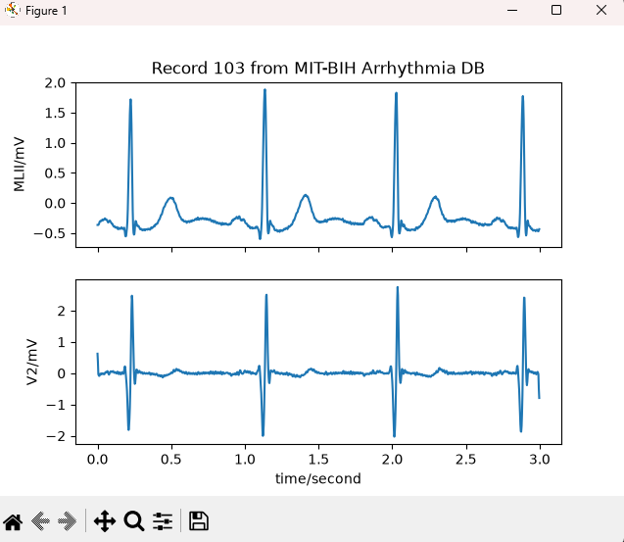
\includegraphics[width=0.75\linewidth]{figure1.png}
    \caption{Extraction of physiological features (Inter-Pulse Intervals) from the MIT-BIH Arrhythmia Database, Record 103.}
    \label{fig:ecg_plot}
\end{figure}

Figure~\ref{fig:ecg_plot} shows the ECG signal processed by the sensors. The QRS complexes are clear and regular, so R-peak detection is reliable. The extracted IPI is about 0.882~s (binary \texttt{.1110000111100}), which corresponds to a heart rate of about 68 beats per minute. Figure~\ref{fig:features} shows the 30 feature vectors generated independently by $S$ and $R$.

\begin{figure}[htbp]
    \centering
    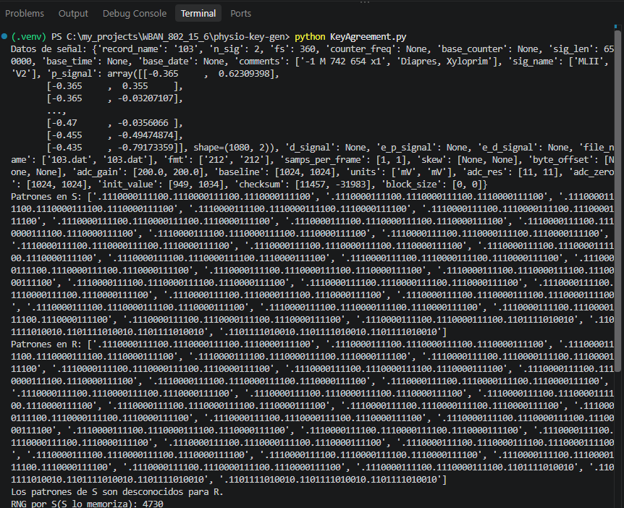
\includegraphics[width=0.85\linewidth]{figure2.png}
    \caption{Terminal output: ECG record metadata and the feature vectors generated by sensors $S$ and $R$.}
    \label{fig:features}
\end{figure}

\subsection{Key Agreement}
\begin{figure}[htbp]
    \centering
    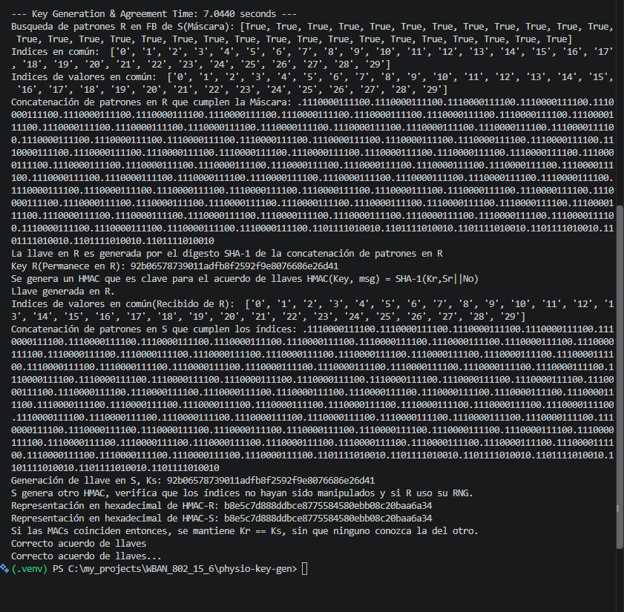
\includegraphics[width=0.85\linewidth]{figure3.png}
    \caption{Terminal output confirming successful local key generation and HMAC matching.}
    \label{fig:terminal_output}
\end{figure}

As shown in Figure~\ref{fig:terminal_output} and Table~\ref{tab:keys}, all 30 features of $R$ passed the Bloom filter test ($|I| = 30 > \tau$). Both sensors generated the identical key and matching HMAC tags without any key transmission, and the final confirmation succeeded.

\begin{table}[htbp]
  \centering
  \caption{Key agreement results (hexadecimal, 160-bit).}
  \label{tab:keys}
  \begin{tabular}{l l}
    \toprule
    \textbf{Value} & \textbf{Result} \\
    \midrule
    Key at $R$, $\Kr$           & \texttt{92b06578739011adfb8f2592f9e8076686e26d41} \\
    Key at $S$, $\Ks$           & \texttt{92b06578739011adfb8f2592f9e8076686e26d41} \\
    $\mathit{MAC}_1$ (from $R$) & \texttt{b8e5c7d888ddbce8775584580ebb08c20baa6a34} \\
    $\mathit{MAC}_2$ (at $S$)   & \texttt{b8e5c7d888ddbce8775584580ebb08c20baa6a34} \\
    Nonce $N_o$                 & 4730 \\
    Final confirmation          & Verified \\
    \bottomrule
  \end{tabular}
\end{table}

\subsection{Bloom Filter Validation}
To check that the Bloom filter meets its design target, we inserted 30 random 42-bit features into a filter with the parameters in Table~\ref{tab:params}. We then queried it with 200\,000 random features that had not been inserted. The original membership test in the repository returned after checking only the first of the $k = 10$ hash positions. Its false-positive rate was 49.5\%, which would let guessed features pass reconciliation half of the time. After we corrected it to check all $k$ positions, the measured rate dropped to 0.093\%, matching the design target (Table~\ref{tab:bloomfp}). The protocol still produced the same key after the fix.

\begin{table}[htbp]
  \centering
  \caption{Measured Bloom filter false-positive rate ($m = 433$, $k = 10$, $n = 30$, 200\,000 probes).}
  \label{tab:bloomfp}
  \begin{tabular}{l c c}
    \toprule
    \textbf{Membership test} & \textbf{False negatives} & \textbf{False-positive rate} \\
    \midrule
    Design target (Eq.~\ref{eq:bloom})   & 0 & 0.096\% \\
    Original: checks only the first hash & 0 & 49.5\% \\
    Corrected: checks all $k$ hashes     & 0 & \textbf{0.093\%} \\
    \bottomrule
  \end{tabular}
\end{table}

\subsection{Execution Time}
The execution time tracker recorded 7.04 seconds for the key generation stage of the Python prototype. This covers loading the ECG record, extracting the IPI features for both sensors, and building the Bloom filter on a desktop computer. Most of the time is spent on file input/output and signal processing in interpreted Python. The cryptographic operations themselves (a few SHA-1 and HMAC computations) take only microseconds. A native implementation on a sensor microcontroller would be considerably faster.
